\chapter{Hidden Gauge Bosons at Lepton-Ion Colliders} \label{bosons}
\vspace{-1cm}
\begin{center}
{\it This chapter is based on work done in Refs.~\cite{Davoudiasl:2023pkq,Davoudiasl:2024fiz}.}
\end{center}
\vspace{1cm}

\section{Introduction}
Most of the results obtained in this dissertation thus far have concerned direct production of particles through an LFV coupling. However, as we have seen in Chapter 2, LFV is a generic feature of many leptophilic new physics models. One class of such models, discussed in Section~\ref{sec:U1_bosons}, is the anomaly-free $U(1)_{L_i - L_j}$ lepton family gauge theories. While these models do not have flavor-violation at the outset, any spontaneous breaking of the $U(1)_{L_i - L_j}$ will lead to LFV processes. Spontaneous symmetry breaking of the abelian symmetry can generically lead to off-diagonal couplings of the gauge boson $A'$ to both the charged and neutral leptons, and the scalars responsible for the symmetry breaking typically exhibit LFV couplings as well.

It is worthwhile to consider whether the $A'$ of these theories can be produced via the production mechanism described in Chapter \ref{upc}. In particular, a prompt decay of such a particle would be rife with SM background, since these gauge bosons mostly decay to $\bar{f}f$, where $f$ is a Standard-Model fermion.\footnote{While $A'\rightarrow \bar{f}f'$ is also often possible, the branching for this relative to $A\rightarrow \bar{f}f$ is suppressed.} However, if the coupling $g$ of the $A'$ is small enough and its mass $m_{A'}$ light enough, the decay of the $A'$ can be come displaced. Indeed, for displacements $d \gtrsim 0.1~{\rm mm}$, we expect there to be no SM background.

One potential issue with production of light particles via $\ell^- A_Z \rightarrow \ell^- A_Z A'$ is that the $A'$ will have high pseudo-rapidity. Beam-dumps have the advantage in this regard, as detectors can be placed directly beyond the target material, allowing detection of displaced decays with $\eta \gg 1$. For colliders such as the EIC or MuSIC discussed in Chapter 4, this is only possible with additional instrumentation far beyond the interaction point. Otherwise, the EIC has $\eta \lesssim 3.5$ and, in line with our assumptions, MuSIC has $\eta \lesssim 6$. While such pseudo-rapidity constraints aren't prohibitive, they do limit the reach of these experiments for detecting displaced particles.

In this chapter, we will explore limits from displaced decays of $U(1)$ gauge bosons at the EIC, MuSIC, and a 1 TeV muon beam dump (MuBeD). For completion, we will consider gauge bosons not only from the $U(1)_{L_i - L_j}$ lepton family symmetries, but also a dark photon and the gauge boson of an abelian $U(1)_{B-L}$ symmetry. In Section \ref{sec:vector_boson_decay}, we will review the branching fractions of the gauge bosons to SM final states. In Section \ref{sec:detector_geom}, we will consider this signal in the context of the geometry of each of the signals, and discuss the requirements necessary to reconstruct the displaced signal. In Sections \ref{sec:vector_EIC_limits} and \ref{sec:vector_MuBeD_MuSIC_limits} we will provide limits on the gauge boson coupling (or kinetic mixing for the dark photon) at the EIC, MuBeD, and MuSIC. Finally, in Section \ref{sec:displaced_vertex_resolution}, we will discuss the reliability of assumptions we have made when analyzing displaced vertices at lepton-ion colliders.


\section{Vector Boson Decay Rates}\label{sec:vector_boson_decay}
The process under consideration is production of a massive vector boson $A'$, represented by the process $\ell^- A_Z \rightarrow \ell^- A_Z A'$. If the $A'$ is light enough, it is likely that its decay will be displaced relative to the production vertex, which yields a signal with virtually zero SM background. For simplicity, we will focus on the scenario in which the $A'$ decays to $e^+ e^-$ at the EIC (taking advantage of the EIC's electron tracking capabilities), and to $e^+e^-$ or $\mu^+\mu^-$ at MuSIC and MuBeD. We only consider emission of the $A'$ from the lepton and not from the ion; emission from the ion will be suppressed by the nuclear form-factor $F(m_{A'}^2)$ except for fairly light $A'$ masses, where other experiments already provide stringent limits. The Feynman diagrams representing the process are shown in Fig.~\ref{fig:production_diagram}. The total cross-sections and kinematic distributions for scalars produced in this way were reviewed in Chapter \ref{upc}. The vector scenario is very similar. 

We will be interested in decays of the hidden vector to SM final states. We assume that these are the only accessible decay modes of the hidden vector. We begin by considering an interaction of the form
\begin{align}
    {\cal L}_{\rm int.} &= -A'_\mu\sum_f Q_f\bar{f}\gamma^\mu\left(g_L P_L + g_R P_R\right)f
\end{align}
which yields a decay rate for $A'\rightarrow \bar{f}f$ (assuming $m_{A'} > 2m_f$)
\begin{align}
    \Gamma(A' \rightarrow \bar{f}f) &= \frac{Q_f^2C_f}{24\pi}m_{A'}\sqrt{1-\frac{4m_f^2}{m_{A'}^2}}\left((g_L^2 + g_R^2)\left(1-\frac{m_f^2}{m_{A'}^2}\right)+6g_Lg_R\frac{m_f^2}{m_{A'}^2}\right)
\end{align}
\begin{table}[]
\centering
\begin{tabular}{@{}cccccc@{}}
\toprule
{\rm charge}        & $U(1)_{\rm EM}$ & $U(1)_{B-L}$ & $U(1)_{L_e - L_\mu}$ & $U(1)_{L_e - L_\tau}$ & $U(1)_{L_\mu - L_\tau}$ \\ \midrule
$Q_e$        & $-1$            & $-1$         & $+1$                 & $+1$                  &\ \ $0$                     \\
$Q_\mu$      & $-1$            & $-1$         & $-1$                 &\ \ $0$                   & $+1$                    \\
$Q_\tau$     & $-1$            & $-1$         &\ \ $0$                  & $-1$                  & $-1$                    \\
$Q_{\nu_e}$    &\ \ $0$             & $-1$         & $+1$                 & $+1$                  &\ \ $0$                     \\
$Q_{\nu_\mu}$  &\ \ $0$             & $-1$         & $-1$                 & $0$                   & $+1$                    \\
$Q_{\nu_\tau}$ &\ \ $0$             & $-1$         &\ \ $0$                  & $-1$                  & $-1$                    \\
$Q_{u_i}$      & $+2/3$          & $+1/3$        &\ \ $0$                  &\ \ $0$                   &\ \ $0$                     \\
$Q_{d_i}$      & $-1/3$          & $+1/3$        &\ \ $0$                  &\ \ $0$                   &\ \ $0$                     \\ \bottomrule
\end{tabular}
\caption{The charges of the SM fermions under each of the anomaly-free abelian groups discussed in the text.}
\label{table:U1_charges}
\end{table}
where $Q_f$ is the charge under the gauge group $U(1)_X$ and $C_f$ is a color factor ($3$ for quarks and $1$ for leptons). A table representing the charges $Q_f$ of the SM fermions $f$ for each of the gauge theories considered is shown in Table~\ref{table:U1_charges}. While we will assume that the $A'$ couples to the vector current for the quarks and charged leptons, whether this is the case for neutrinos depends on whether the neutrinos are Dirac or Majorana fermions. If they are Dirac, then then $\nu_L$ and $\nu_R$ carry the same mass, so one can package them into a Dirac spinor and take $g_L = g_R = g_X$. Otherwise, $\nu_L$ and $\nu_R$ must be treated separately, with $\nu_R$ generically much heavier than $\nu_L$. This scenario corresponds to $g_L = g_X$ and $g_R = 0$ or vice versa, as the interaction must contain a left- or right-handed projection operator to treat each field separately.\footnote{One could still package them into a Dirac spinor, but this is inconvenient since there is a mass splitting between the left- and right-handed components of the spinor.} While a Majorana mass term violates the $U(1)_{B-L}$ and $U(1)_{L_i - L_j}$ symmetries, such a term often arises alongside the spontaneous breaking of said symmetries due to interaction with a charge $\pm2$ scalar which acquires a VEV \cite{Mohapatra:1980qe}. Given the predictive power of a Majorana mass term for the right-handed neutrino in describing the observed neutrino masses, we will assume that this is the case. Then, the decay rate to neutrinos is
\begin{figure}[t!]
    \centering
    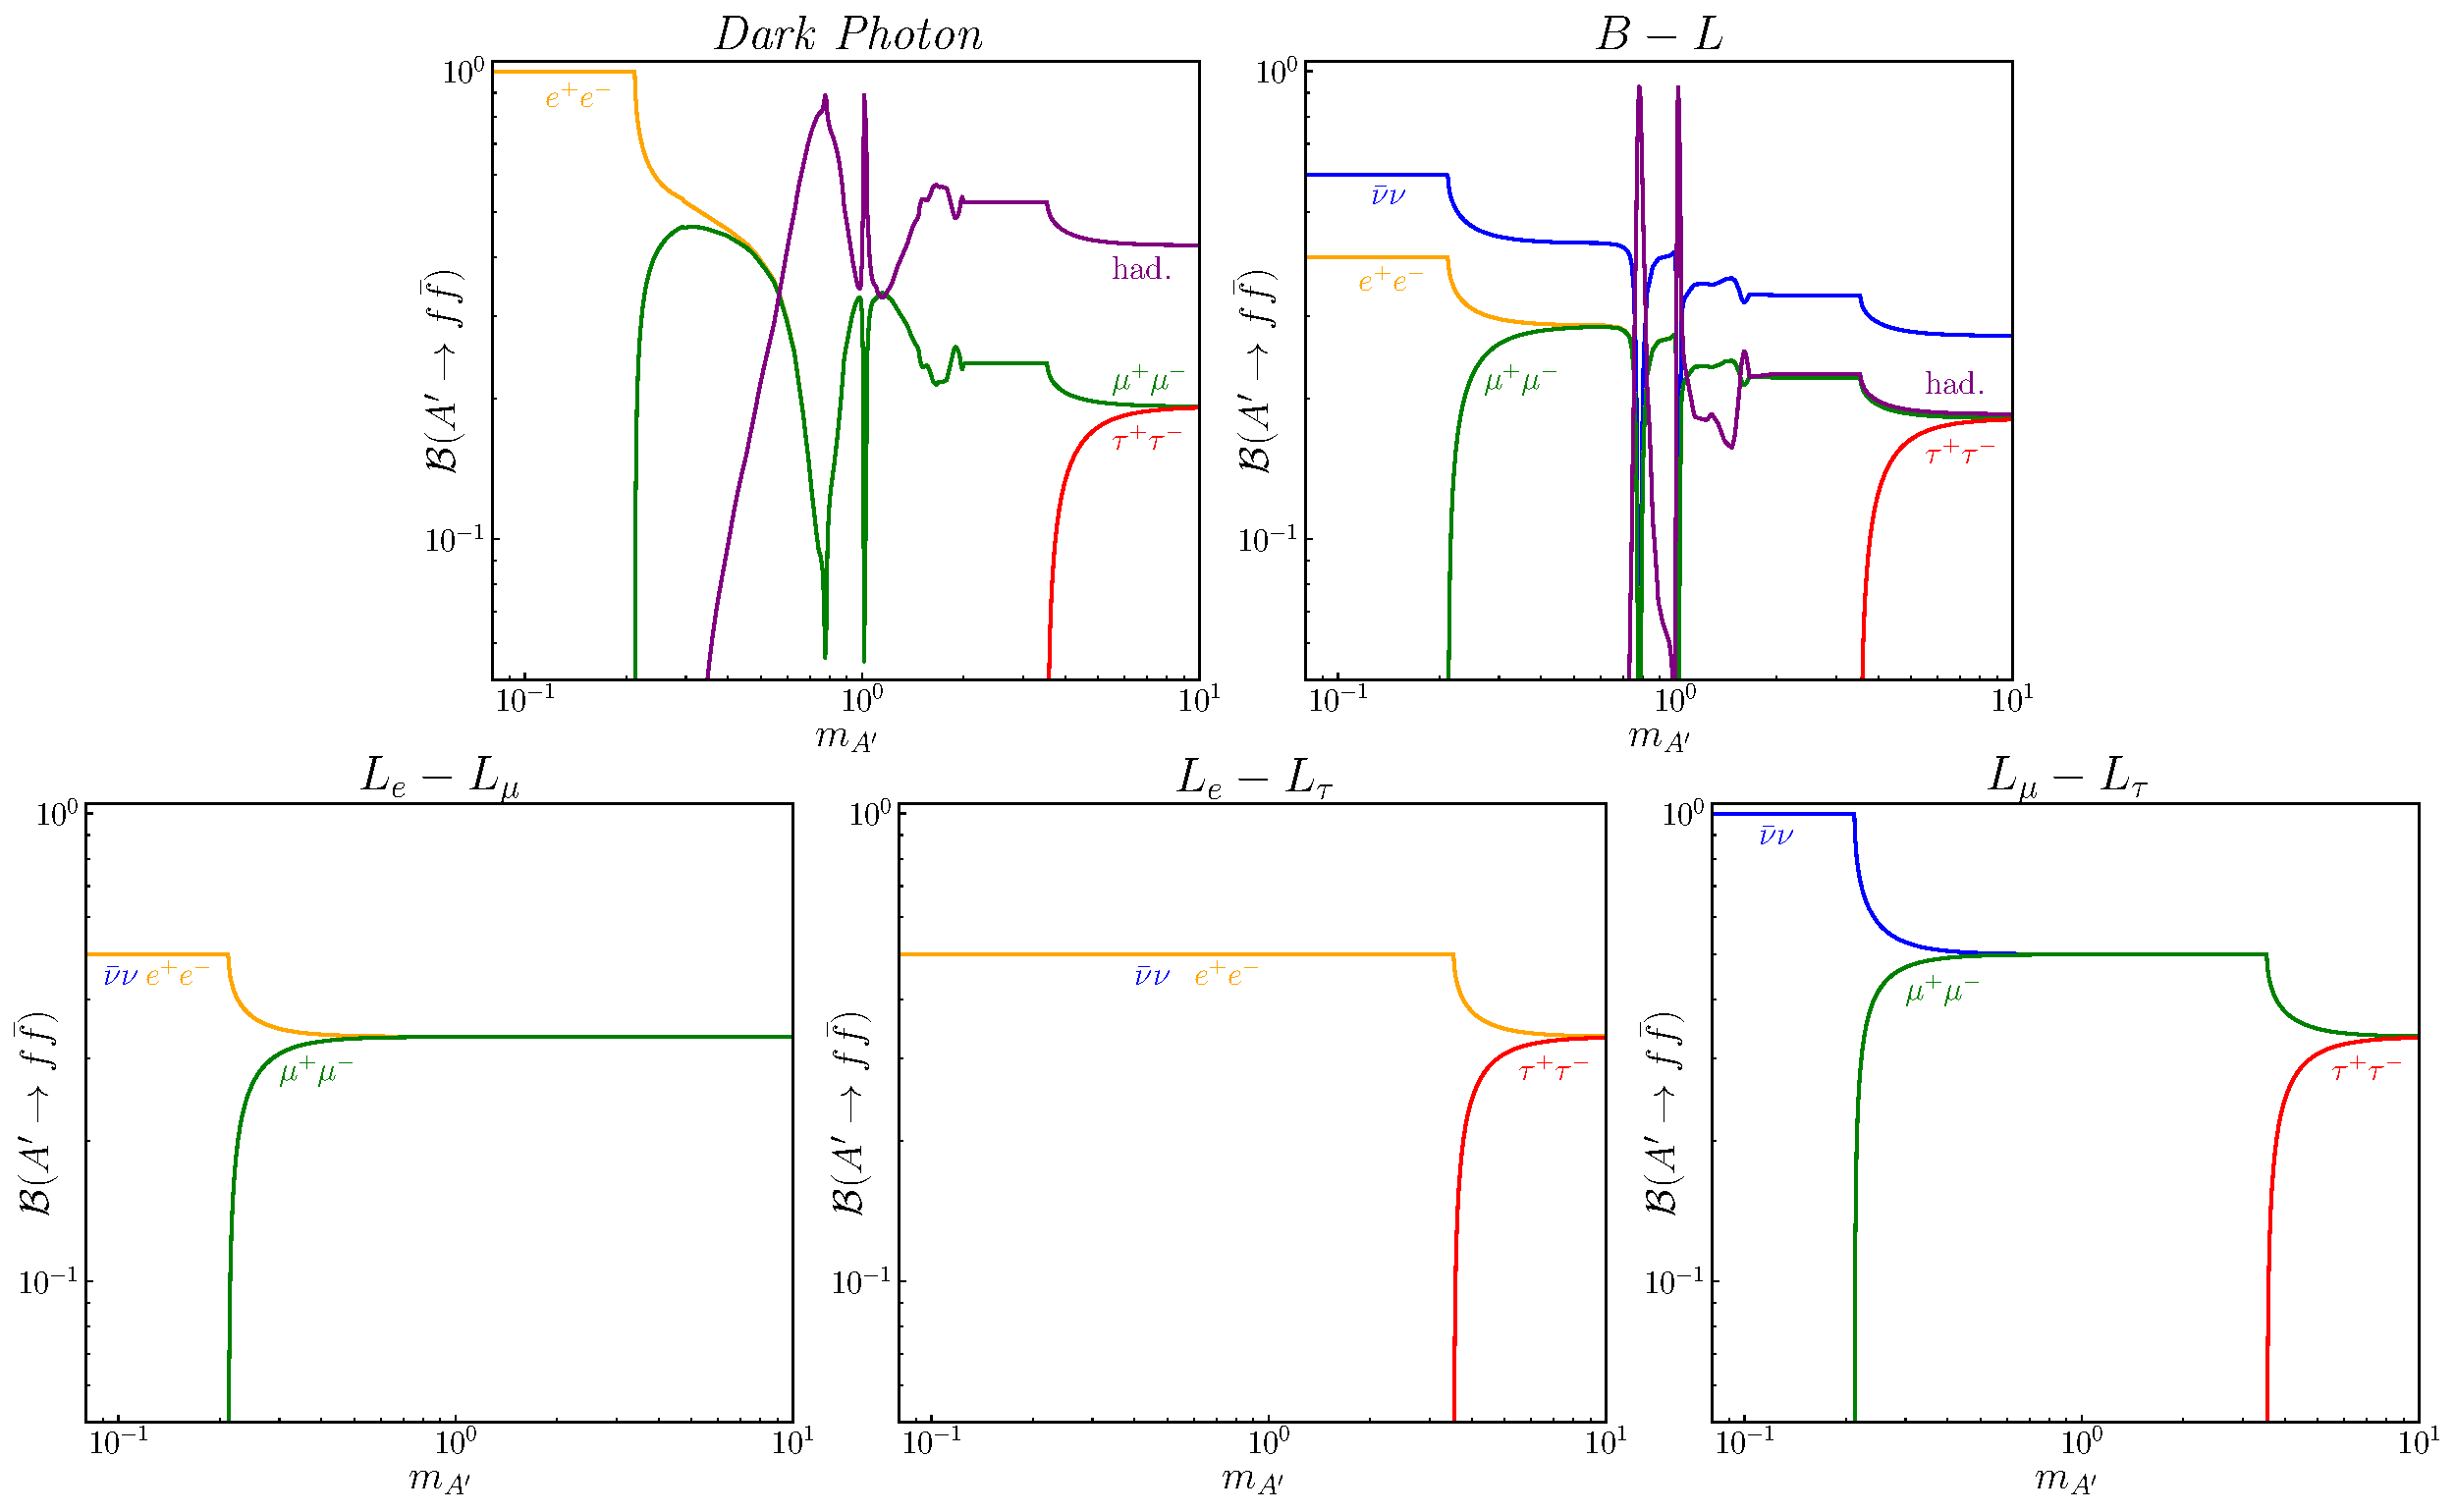
\includegraphics[width=\linewidth]{figures/chapter6/gauge_boson_branching_fractions.pdf}
    \caption{Branching fractions of a dark photon and anomaly-free $U(1)_X$ gauge bosons into SM final states.}
    \label{fig:gauge_boson_branching_fractions}
\end{figure}

\begin{align}
    \Gamma(A' \rightarrow \bar{\nu}_\ell\nu_\ell) &\approx \frac{g_X^2Q_{\nu_\ell}^2}{24\pi}m_{A'}
\end{align}
whereas the decay rate to charged leptons is
\begin{align}
    \Gamma(A' \rightarrow \bar{\ell}\ell) &= \frac{g_X^2Q_\ell^2}{12\pi}m_{A'}\left(1+\frac{2m_\ell^2}{m_{A'}^2}\right)\sqrt{1-\frac{4m_\ell^2}{m_{A'}^2}}.
\end{align}
 The decay rate to quark final states is less straightforward due to the nonperturbative nature of the strong interaction. In this case, Ref.~\cite{Ilten:2018crw} computes the decay rate of the $A'$ to hadrons using the ${\cal R}$-ratio for dark photons, and uses a combination of vector meson dominance and a more general data-driven approach to recast the rate for other gauge bosons. For our purposes, we digitize the rates for the dark photon and $U(1)_{B-L}$ gauge boson from Fig.~9 of Ref.~\cite{Ilten:2018crw}. 
The plots of the branching fractions to neutrinos, hadrons, and each charged lepton are shown in Fig.~\ref{fig:gauge_boson_branching_fractions}.

\section{Detector Geometry and Displaced Signal}\label{sec:detector_geom}
Here, we review the expected detector requirements and geometry for the EIC, as well as reasonable assumptions for MuSIC and MuBeD. In general, we can parameterize the number of signal events in terms of the differential production cross-section $d\sigma/d\gamma\,d\eta$ as follows:
\begin{align}
    N_{\rm sig.} &= {\cal L}\int{d\gamma\int_{\eta_{\rm min}}^{\eta_{\rm max}}{d\eta\left\{\frac{d\sigma}{d\gamma\,d\eta}P_{\rm disp.}\,\sum_{X}\epsilon_X {\cal B}(A'\rightarrow X)\right\}}}\label{eq:N_sig}
\end{align}
where ${\cal L}$ is the luminosity, $\gamma$ and $\eta$ represent the boost and pseudo-rapidity of the produced vector boson $A'$, and $\epsilon_X$ is the efficiency of detecting the final-state $X$. Here, $P_{\rm disp.}$ denotes the probability that the $A'$ decays in a region of the detector apparatus for which it is possible to discern that its decay products are displaced. For the situations that we consider, we take it to be given by
\begin{align}
    P_{\rm disp.} = e^{-d_{\rm min}/\gamma c \tau_{\tiny A'}} - e^{-d_{\rm max}/\gamma c \tau_{\tiny A'}}\label{eq:pdisp}
\end{align}
where  $d_{\rm min}$ and $d_{\rm max}$ are the minimum and maximum distances for which a displaced decay can be resolved, and $\tau_{A'}$ is the rest-frame lifetime of the $A'$. While $d_{\rm min}$ and $d_{\rm max}$ are straightforward parameters in a fixed-target experiment, they can depend greatly on the kinematics of the final-state decay products in collider experiments. Rather than focusing directly on the kinematics of the decay products, we operate under the assumption that $\eta_{X} \approx \eta_{A'}$\footnote{For leptonic final-states, the opening angle $\theta_{\ell\ell} \approx 2/\gamma \ll 1$ for most of the parameter space considered, so this is a reasonable assumption.} and $E_X \approx E_{A'}/2$. We note that the detection efficiencies $\epsilon_X$ in principle depend on the kinematics of the SM final states, but we take them to be constant for simplicity. We will focus on leptonic final-states, so $X = \ell^+\ell^-$ for $\ell = e$ or $\ell = \mu$.


\begin{center}
    {\it 1. EIC}
\end{center}
We will assume that the EIC has excellent electron detection capabilities, but will ignore the possibility of muon reconstruction. Hence, we take $\epsilon_e = 100\%$ and $\epsilon_\mu = 0\%$. Then, the main difficulty in computing \ref{eq:N_sig} is determining the minimum and maximum resolvable displacements at the EIC.

To determine $d_{\rm min}$, we refer to the design document for the ECCE detector (now the ePIC Collaboration) at the EIC \cite{Adkins:2022jfp}, which provides resolutions for the two-dimensional (2D) distance of closest approach (${\rm DCA}_{\rm 2D}$) of pions. In particular, ${\rm DCA}_{\rm 2D}^{\rm min} = 100~{\rm \mu m}$ for almost all track transverse momenta and pseudorapidities. If we adopt this as the resolution for the ${\rm DCA}_{\rm 2D}$ for the electrons at the EIC, we can relate $d_{\rm min}$ to the lifetime $\tau_{A'}$ of the $A'$. In particular, the transverse DCA is defined as the spatial separation between the primary vertex and reconstructed particle paths projected onto the transverse plane (see Fig.~\ref{fig:DCA2D}). We take the opening angle of the final-state leptons to be $\theta_{\ell\ell}$, and assume that each lepton has angle $\theta_{\ell\ell}/2$ w.r.t. the direction of the vector boson. In the limit of $m_{A'} \gg m_e$, this corresponds to $\theta_{\ell\ell} \sim 2v/\gamma$, where $v$ and $\gamma$ are the speed and boost of the vector boson in the lab frame. Assuming $m_e \ll m_{A'}$, we find $d_{\rm min} \approx \gamma({\rm DCA}_{\rm 2D}^{\rm min})/v \cos{\theta}$, where $\theta$ is the angle the vector boson makes with the beam axis in the laboratory frame. The details are provided in Appendix~\ref{dca_appendix}.

\begin{figure}[t!]
    \centering
    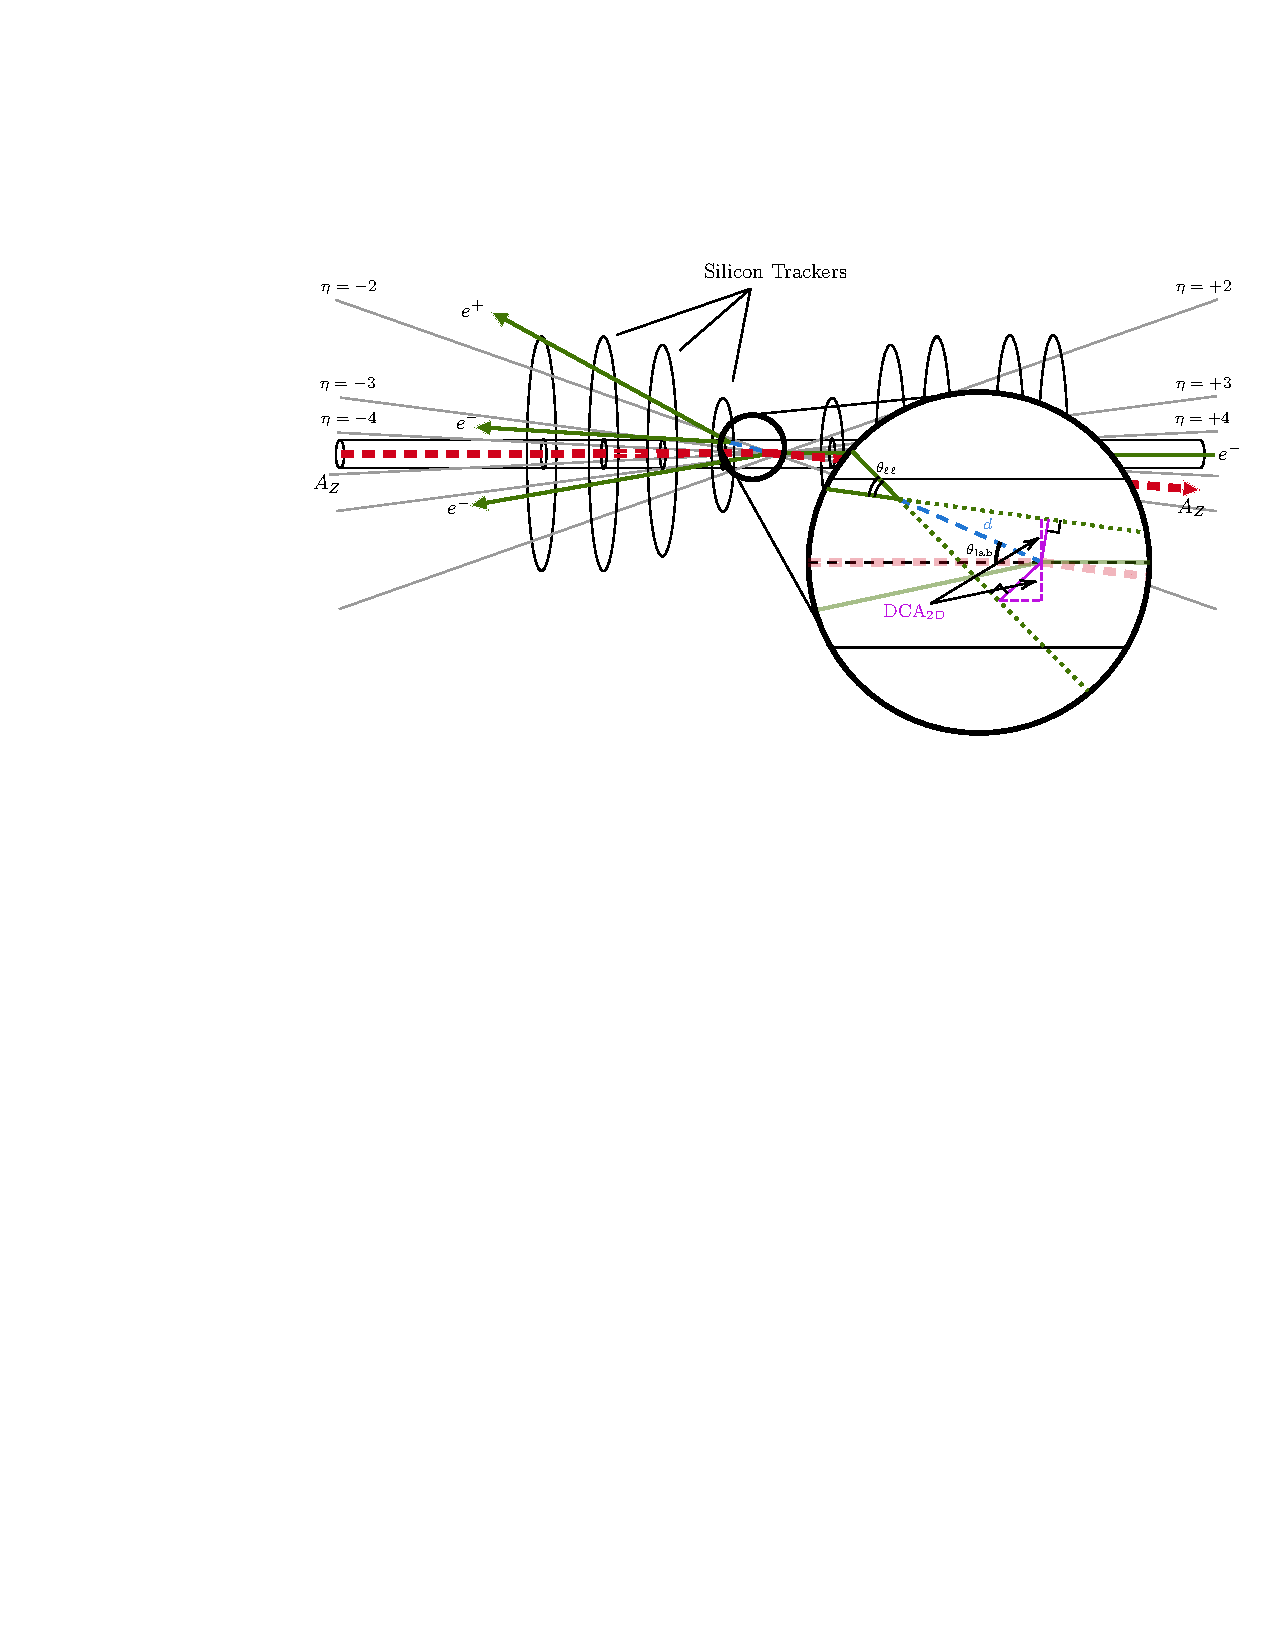
\includegraphics[width=0.9\linewidth]{figures/chapter6/DCA2D_ePIC.pdf}
    \caption[A schematic representing the proposed ePIC detector at the EIC, along with a depiction of the distance-of-closest approach.]{A schematic representation of the displaced process under consideration, including a diagram the transverse distance-of-closest-approach (${\rm DCA}_{\rm 2D}$) for the final-state decay $e^+e^-$ products of a vector boson with displacement $d$ at the EIC. The tracks of the electrons and positrons in the final-state are shown as solid green lines, and the reconstructed tracks of the $e^+e^-$ decay products from the dark boson are shown as dashed green lines. The distance-of-closest-approach for each decay product is depicted as a solid magenta line, and its transverse component (the ${\rm DCA}_{\rm 2D}$) is depicted as a vertical dashed magenta line. The size of the beam-pipe and placement of the silicon tracker is reproduced from Ref.~\cite{Adkins:2022jfp}. In order to ensure each track can be reconstructed with the desired precision, we require that the vector boson decays before the first silicon tracker, which is placed $25~{\rm cm}$ from the interaction point.}
    \label{fig:DCA2D}
\end{figure}

Determination of $d_{\rm max}$ is more straightforward. Referring again to Ref.~\cite{Adkins:2022jfp}, the tracking region consists of nine silicon trackers roughly evenly spaced in the region $|z| < 1~{\rm m}$ and $|\eta| < 3.5$, with the first trackers at $|z| = 25~{\rm cm}$, where $z$ is the position along the beam-axis from the interaction point (as illustrated in Fig.~\ref{fig:DCA2D}). In order to determine that the electron and positron decay products are displaced, it is crucial that their trajectories can be adequately reconstructed, so we require that the $A'$ decays with $|\eta| < 3.5$ {\it before} it reaches the first silicon tracker. This corresponds to a maximum resolvable displacement of $d_{\rm max} = (25~{\rm cm})/\cos{\theta}$. It is possible that a determination can be made as to whether the decay products are displaced with fewer trackers involved, but we find negligible difference in our results choosing $z_{\rm max} = 25~{\rm cm}$ or $z_{\rm max} = 1~{\rm m}$. 

One of the main limiting factors of our production cross-section is the production of dark photons with far-backward pseudorapidities ($\eta < -3.5$) which are beyond the EIC's current tracking capabilities. Notably, the ECCE/ePIC detector proposal includes a far-forward detector, the B0 spectrometer, with the capability to track particles with $4 < \eta < 6$. Thus, we consider a scenario in which a similar detector is installed in the backward region at around $z = -5~{\rm m}$,\footnote{The precise location is not crucial, so long as it is far enough away that it can track those decay products of the $A'$ with large pseudorapidities; we simply make this choice for a direct comparison to the B0 spectrometer.} with the ability to track electrons with $-6 < \eta < -4$. We assume that this detector has a weaker DCA resolution than the rest of the detector given its distance from the interaction point, taking ${\rm DCA}_{\rm 2D}^{\rm min} = 200\,\mu{\rm m}$.

For such vector bosons, a concerning background is ordinary photon conversion. However, because our signal is concentrated at large $|\eta|$ in the direction of the electron beam, the vast majority of signal events will occur in a region of the proposed ECCE/ePIC detector which is very sparse. As a result, cutting away displaced vertices which originate at the silicon disks or on the beam-pipe should be sufficient for avoiding this background while minimally affecting the number of signal events. Reconstruction of the invariant mass of lepton pairs could be another experimental handle to distinguish $A'$ events from photon conversions in order to satisfy our assumption of negligible SM background.

Another potential source of background is misidentification of charged pions, which will be copiously produced in ion collisions, as $e^\pm$. However, in the electron end cap where our signal is concentrated, the fake rate is quite low, approximately $10^{-4}$. Since our signal requires both $e^-$ and $e^+$ as well as the displaced vertex, this background should be negligible. 

Finally, there is also the possibility of signal reduction if electrons and positrons from the $A'$ decay are lost down the beam pipe. We have used our kinematic distributions with some simplifying assumptions to estimate that, conservatively, this rate is no larger than $20\%-30\%$ even with the signal strongly collimated in the backward direction. Since our estimate is somewhat crude (and would not affect our projections significantly), we do not include it in our projections, but a future study with a full Monte Carlo detector simulation could take this possibility into account for more accurate bounds. 

\begin{center}
    {\it 2. MuSIC}
\end{center}

We repeat the analysis for the EIC but with MuSIC, assuming an integrated luminosity of ${\cal L} = 400/A \approx 2~{\rm fb}^{-1}$ over the course of 10 years. As in earlier chapters, we assume the main detector apparatus at MuSIC has a pseudo-rapidity range of $|\eta | < 6$. We additionally consider a far-backward scenario, in which there is tracking instrumentation in the region $6 < |\eta| < 8$. This will allow for a considerable increase in reach, given the anticipated pseudorapidity distributions at MuSIC (see Section \ref{sec:phi_kin}). Such a reach in pseudorapidity would require instrumentation many meters away from the interaction point, so we take a maximum displacement of $z_{\rm max} \approx 30~{\rm m}$. Like the EIC, we assume that MuSIC will only be able to resolve displaced vertices for particles whose reconstructed trajectories exceed some minimum transverse DCA, ${\rm DCA}_{\rm 2D}^{\rm min}$, from the interaction point. For the region $|\eta| < 6$, we assume a transverse DCA resolution of ${\rm DCA}_{\rm 2D}^{\rm min} = 200~{\mu \rm m}$, in line with our assumption for the far-backward scenario at the EIC (which has a similar pseudo-rapidity requirement). For the far-backward scenario at MuSIC, we anticipate that the transverse DCA resolution will worsen considerably for $|\eta| < 8$, at which point the reconstructed trajectories will be many meters long. Hence, we will take a minimum DCA resolution of ${\rm DCA}_{\rm 2D}^{\rm min} = 1~{\rm mm}$.

\begin{center}
    {\it 3. MuBeD}
\end{center}

For the muon beam dump scenario, we assume a $1~{\rm TeV}$ muon beam, then repeat the analysis performed in  Refs.~\cite{Cesarotti:2022ttv,Cesarotti:2023sje}. The set-up is shown in Fig.~\ref{fig:MuBeD}. Once again, the number of vector boson production events in the thin-target approximation is
\begin{align}
    \frac{dN_{\rm prod.}}{dE_k\,d\theta_k\,dz} &= \frac{N_\mu \rho_{\rm tar}}{M_{\rm tar}}\int_0^{L_{\rm tar}}d\ell \frac{d\sigma}{dE_k\,d\theta_k}\frac{dP(z-\ell)}{dz}\nonumber\\
    &= N_\mu\frac{\rho_{\rm tar}L_{\rm tar}}{M_{\rm tar}}\frac{d\sigma}{dE_k\,d\theta_k}\frac{P(z) - P(z - L_{\rm tar})}{L_{\rm tar}}
\end{align}
\begin{figure}[t!]
    \centering
    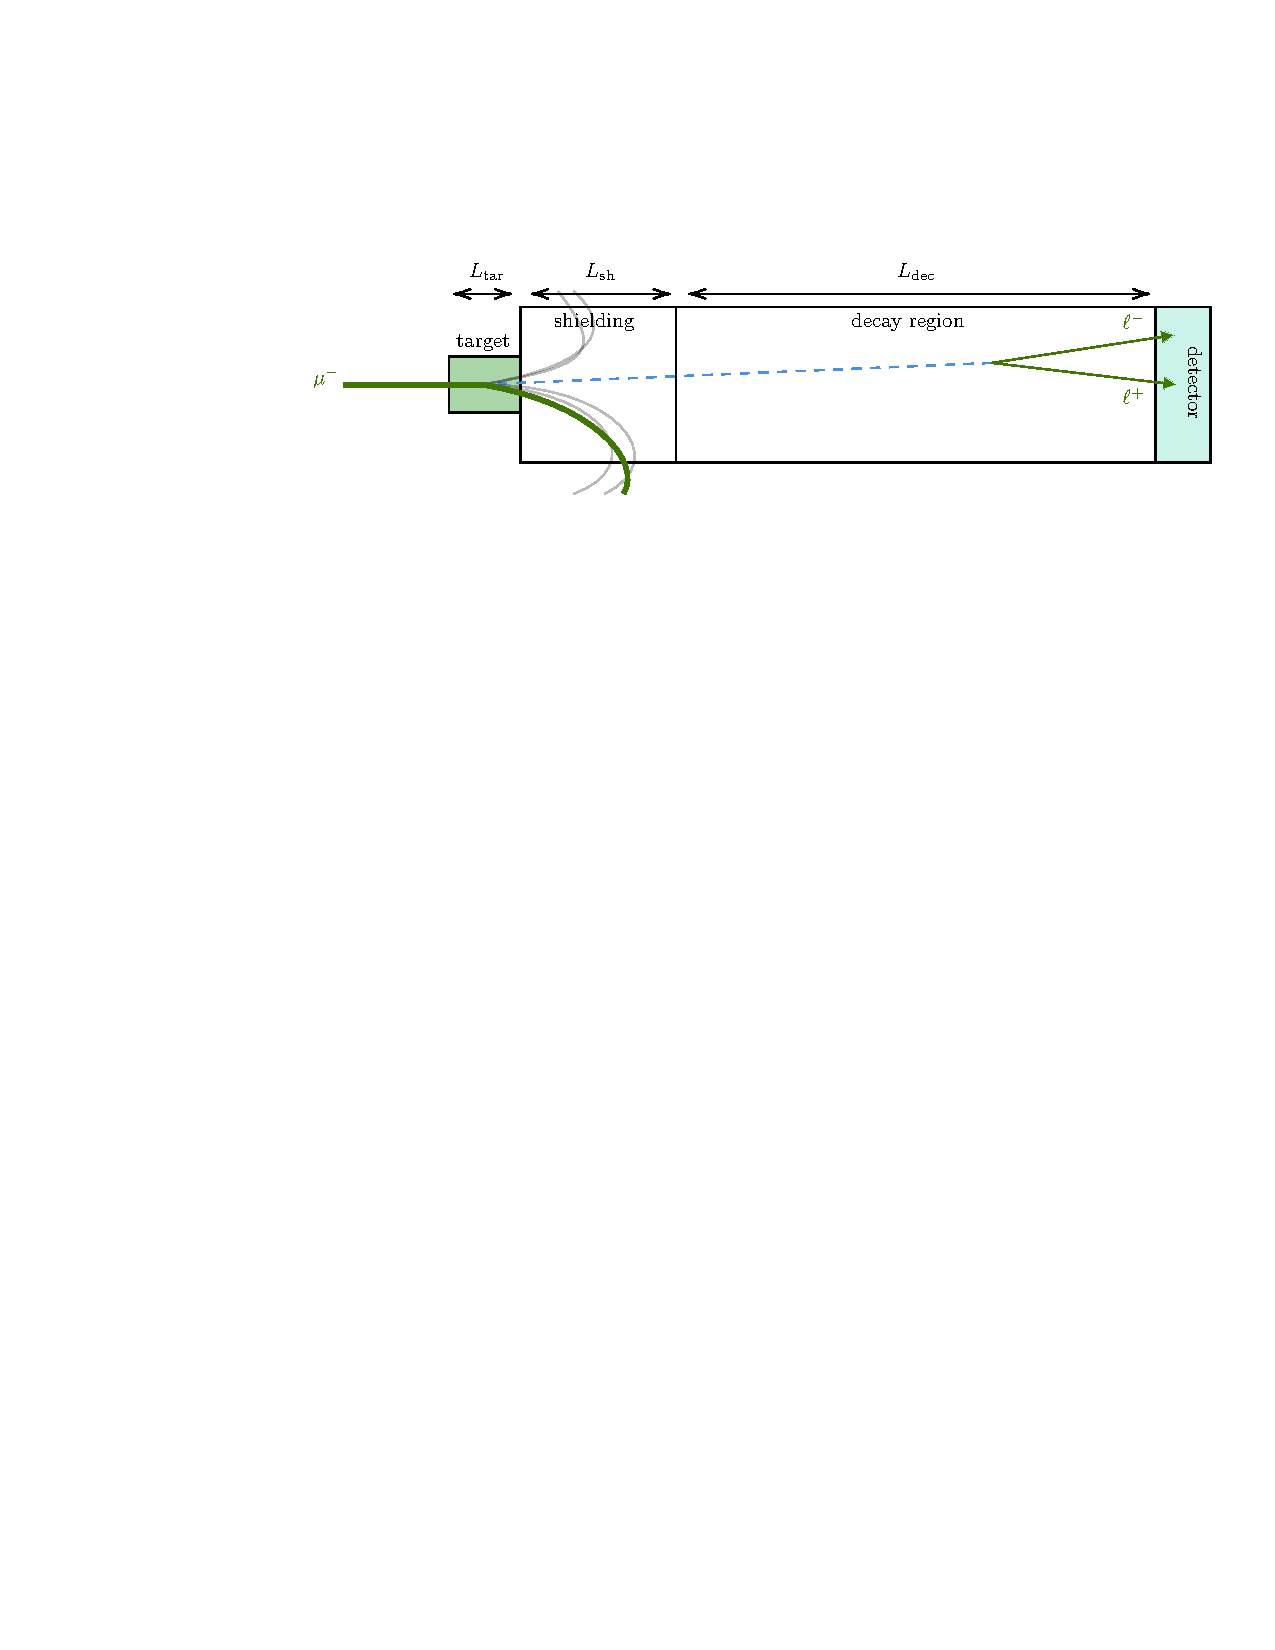
\includegraphics[width=0.9\linewidth]{figures/chapter6/muon_beam_dump.pdf}
    \caption[A schematic depiction of a muon beam dump experiment.]{A schematic depiction of a muon beam dump experiment. The muon beam collides with the target (length $L_{\rm tar})$, producing a long-lived vector boson. All charged Standard-Model particles are deflected in the shielding region (length $L_{\rm sh}$), and the vector decays in the decay region (length $L_{\rm dec}$). Finally, the SM decay products of the vector are detected in the detector placed beyond the decay region. Recreated from Ref.~\cite{Cesarotti:2023sje}.}
    \label{fig:MuBeD}
\end{figure}
where we have included a differential w.r.t. $\theta_k$ so that we can get the number of signal events into the form (\ref{eq:N_sig}). In this case, while we have assumed the target is small relative to the decay length of the material, we can no longer assume that the decay is prompt; i.e. $\gamma c \tau \ll L_{\rm tar}$. The probability that the boson decays between the shielding region $(z \approx L_{\rm tar} + L_{\rm sh}$) and the detector region ($z\approx L_{\rm tar} + L_{\rm sh} + L_{\rm det}$) is 
\begin{align}
    P_{\rm disp.} &= \int_{L_{\rm tar} + L_{\rm sh}}^{L_{\rm tar} + L_{\rm sh} + L_{\rm det}}\frac{dz}{L_{\rm tar}}\left[\left(1 - e^{-z/\gamma c \tau_{A'}}\right) - \left(1 - e^{-(z-L_{\rm tar})/\gamma c \tau_{A'}}\right)\right]\nonumber \\
    &= \int_{L_{\rm tar} + L_{\rm sh}}^{L_{\rm tar} + L_{\rm sh} + L_{\rm det}}\frac{dz}{L_{\rm tar}}\left[e^{-(z-L_{\rm tar})/\gamma c \tau_{A'}} - e^{-z/\gamma c \tau_{A'}}\right] \nonumber\\
    &= \frac{\gamma c \tau_{A'}}{L_{\rm tar}}\left(1 - e^{-L_{\rm tar}/\gamma c \tau_{A'}}\right)\left(1 - e^{-L_{\rm det}/\gamma c \tau_{A'}}\right)e^{-L_{\rm sh}/\gamma c \tau_{A'}}
\end{align}
While this looks considerably more complicated than the probability of a displaced decay in Eq.~\ref{eq:pdisp}, we can make the additional approximation that $L_{\rm tar} \ll \gamma c \tau_{A'}$. Then, we have
\begin{align}
    P_{\rm disp.} &= e^{-(L_{\rm sh} + L_{\rm det})/\gamma c \tau_{A'}} - e^{-L_{\rm sh}/\gamma c \tau_{A'}}.
\end{align}
In line with the $1.5~{\rm TeV}$ scenario in Refs.~\cite{Cesarotti:2022ttv,Cesarotti:2023sje}, we take $L_{\rm tar} = 5.0~{\rm m}$, $L_{\rm sh} = 10.0~{\rm m}$, $L_{\rm dec} = 100.0~{\rm m}$, and $|\eta| \gtrsim 5$. However, we assume a beam energy of $1~{\rm TeV}$ rather than $1.5~{\rm TeV}$ for a more direct comparison to MuSIC. Defining the effective integrated luminosity to be ${\cal L}_{\rm eff} \equiv N_\mu (\rho_{\rm tar}L_{\rm tar}/M_{\rm tar})$, we recover the form (\ref{eq:N_sig}) for the total number of signal events. In terms of final-states, we assume that the detector apparatus is well-instrumented to detect displaced decays of the gauge boson to $e^+e^-$ and  $\mu^+\mu^-$ with $100\%$ efficiency.



\section{Limits at the EIC}\label{sec:vector_EIC_limits}

We compute $95\%$ C.L. limits on the coupling of the gauge boson $g_X$ at the EIC by computing those values of $g_X$ for which $N_{\rm sig.}(g_X) > 3.09$ \cite{Feldman:1997qc}. For a given mass, there are typically two $g_X$ for which $N_{\rm sig.} = 3.09$, and hence the corresponding limits will be double-sided. If $g_X$ is too large, the lifetime of the $A'$ is too large for the decay to be considered displaced; if $g_{X}$ is too small, then either the cross-section is too small to produce $A'$ at a detectable rate, or the majority of produced $A'$ live too long to decay inside the detector. 


\begin{figure}[t!]
    \centering
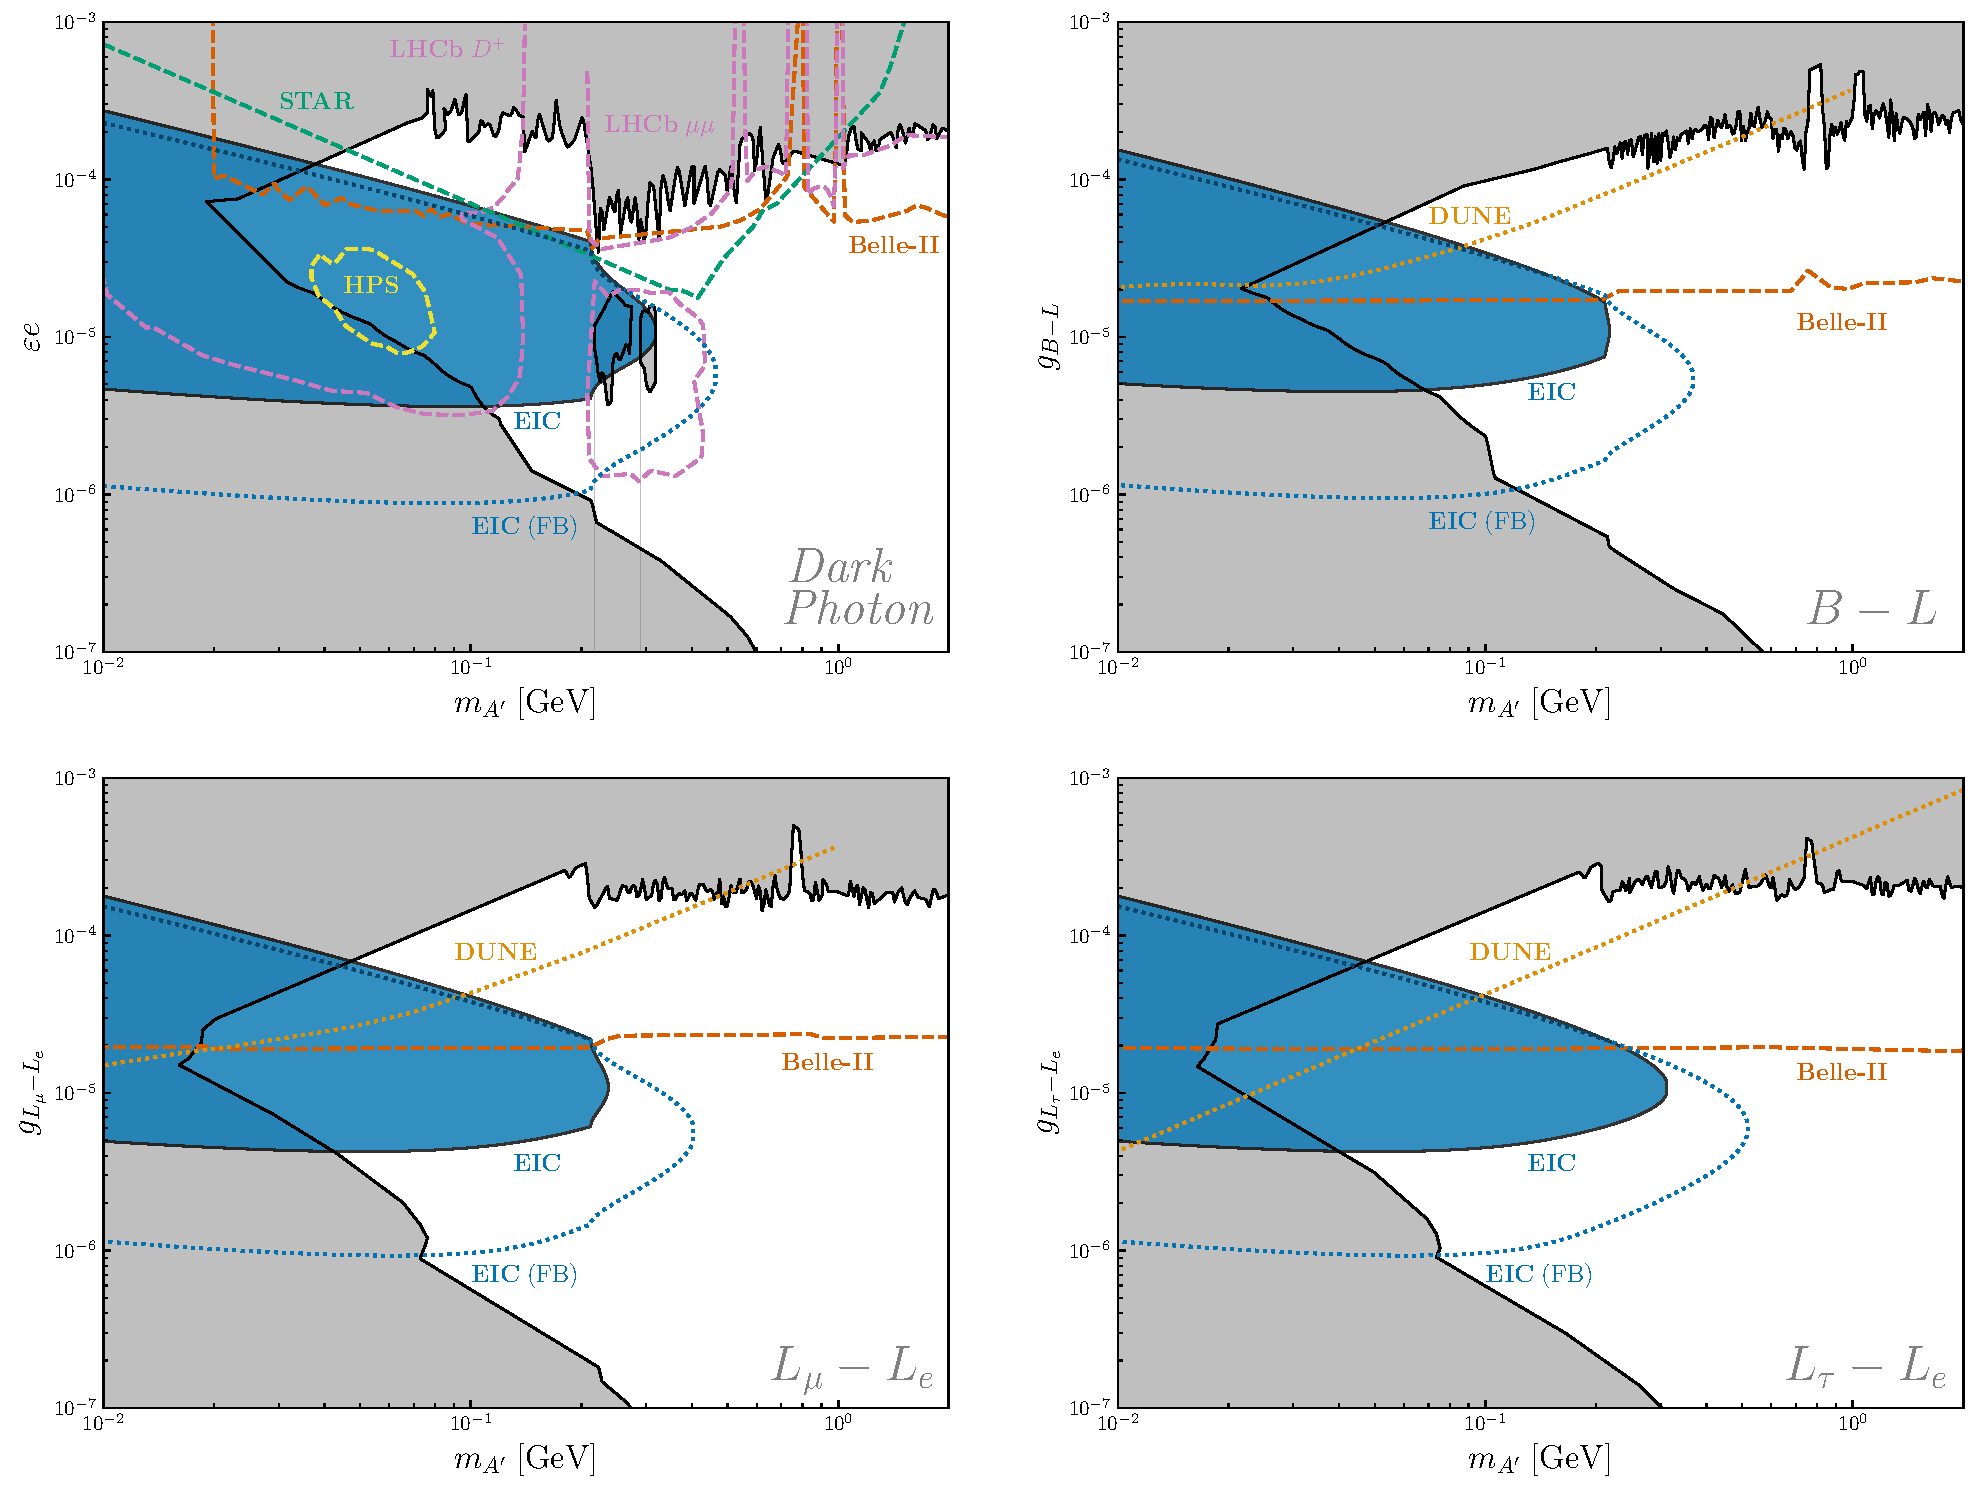
\includegraphics[width=\linewidth]{figures/chapter6/dark_bosons_EIC.pdf}
    \caption[Projected constraints at the EIC on the kinetic mixing of a dark photon and gauge strength of anomaly-free abelian theories.]{Projected constraints  (95\% C.L.) at the EIC on the kinetic mixing of a dark photon (top left), and gauge coupling for a $U(1)_{B-L}$ (top right), $U(1)_{L_\mu - L_e}$ (bottom left), and $U(1)_{L_\tau - L_e}$ (bottom right) vector boson. The blue filled region corresponds to the sensitivity at the EIC assuming a pseudorapidity resolution of $|\eta| < 3.5$, whereas the dotted blue line considers a ``far-backward'' scenario in which the electron-side of the EIC is instrumented for pseudo-rapidity coverage $4 < |\eta| < 6$. Exclusion limits and projections are mostly reproduced from Ref.~\cite{Bauer:2018onh}, but updated to reflect the current state of experiments. The exclusion limits (filled gray region) include U70/NuCal \cite{Blumlein:2011mv,Blumlein:2013cua}, Orsay \cite{Davier:1989wz}, E137 \cite{Bjorken:1988as}, E141 \cite{Riordan:1987aw}, E774 \cite{Bross:1989mp}, NA48 \cite{NA482:2015wmo},  BaBar \cite{BaBar:2009lbr,BaBar:2014zli}, KLOE \cite{KLOE-2:2011hhj,KLOE-2:2012lii,KLOE-2:2016ydq}, LHCb \cite{LHCb:2017trq}, Borexino \cite{Harnik:2012ni}, Texono \cite{Lindner:2018kjo}, NA64 \cite{Banerjee:2019pds} and FASER \cite{FASER:2018eoc}. Projections from current experiments (dashed lines) are shown from STAR \cite{Xu:2022qme}, Belle II \cite{Belle-II:2018jsg}, HPS \cite{Baltzell:2022rpd}, and LHCb \cite{Ilten:2015hya,Ilten:2016tkc}. We also shown projections from DUNE as a dotted line \cite{Wise:2018rnb}. For a more comprehensive set of projected bounds for dark photons, we refer to the Snowmass White Paper \cite{Batell:2022dpx}.}
    \label{fig:dark_bosons_EIC}
\end{figure}



In Fig \ref{fig:dark_bosons_EIC}, we show our projected limits at the 95\% C.L. for displaced dark photons, as well as the gauge bosons for $B-L$, $L_e - L_\tau$ and $L_\mu - L_\tau$. We also show for comparison various existing limits (gray shaded region) and projected limits from current experiments (dashed lines) and future proposed experiments (dotted lines). These are mostly digitized from Ref.~\cite{Bauer:2018onh} using DigitizeIt \cite{DigitizeIt}, although a few additional constraints and projections are included. The blue filled region shows our baseline projection using the ePIC detector and a luminosity for gold ion collisions of ${\cal L} = 100~{\rm fb}^{-1} / A$. We see that the EIC can provide significant new constraints on the parameter space for masses $m_{A'} \sim 100~{\rm MeV}$ and moderately weak couplings $g_{X} \sim 10^{-5}$ for each of the considered bosons. Even comparing to other projected experimental bounds, the EIC provides useful reach in this parameter space. The blue dotted line labeled ``EIC (FB)'' shows how the projected bounds from the EIC could be improved by the inclusion of a far-backward detector in the direction of the electron beam, as described above. The additional pseudo-rapidity coverage up to $|\eta| < 6$ expands the mass reach to $400~{\rm MeV}$, for a coupling of $g_{X} \sim 10^{-5}$.



\begin{figure}[t!]
    \centering
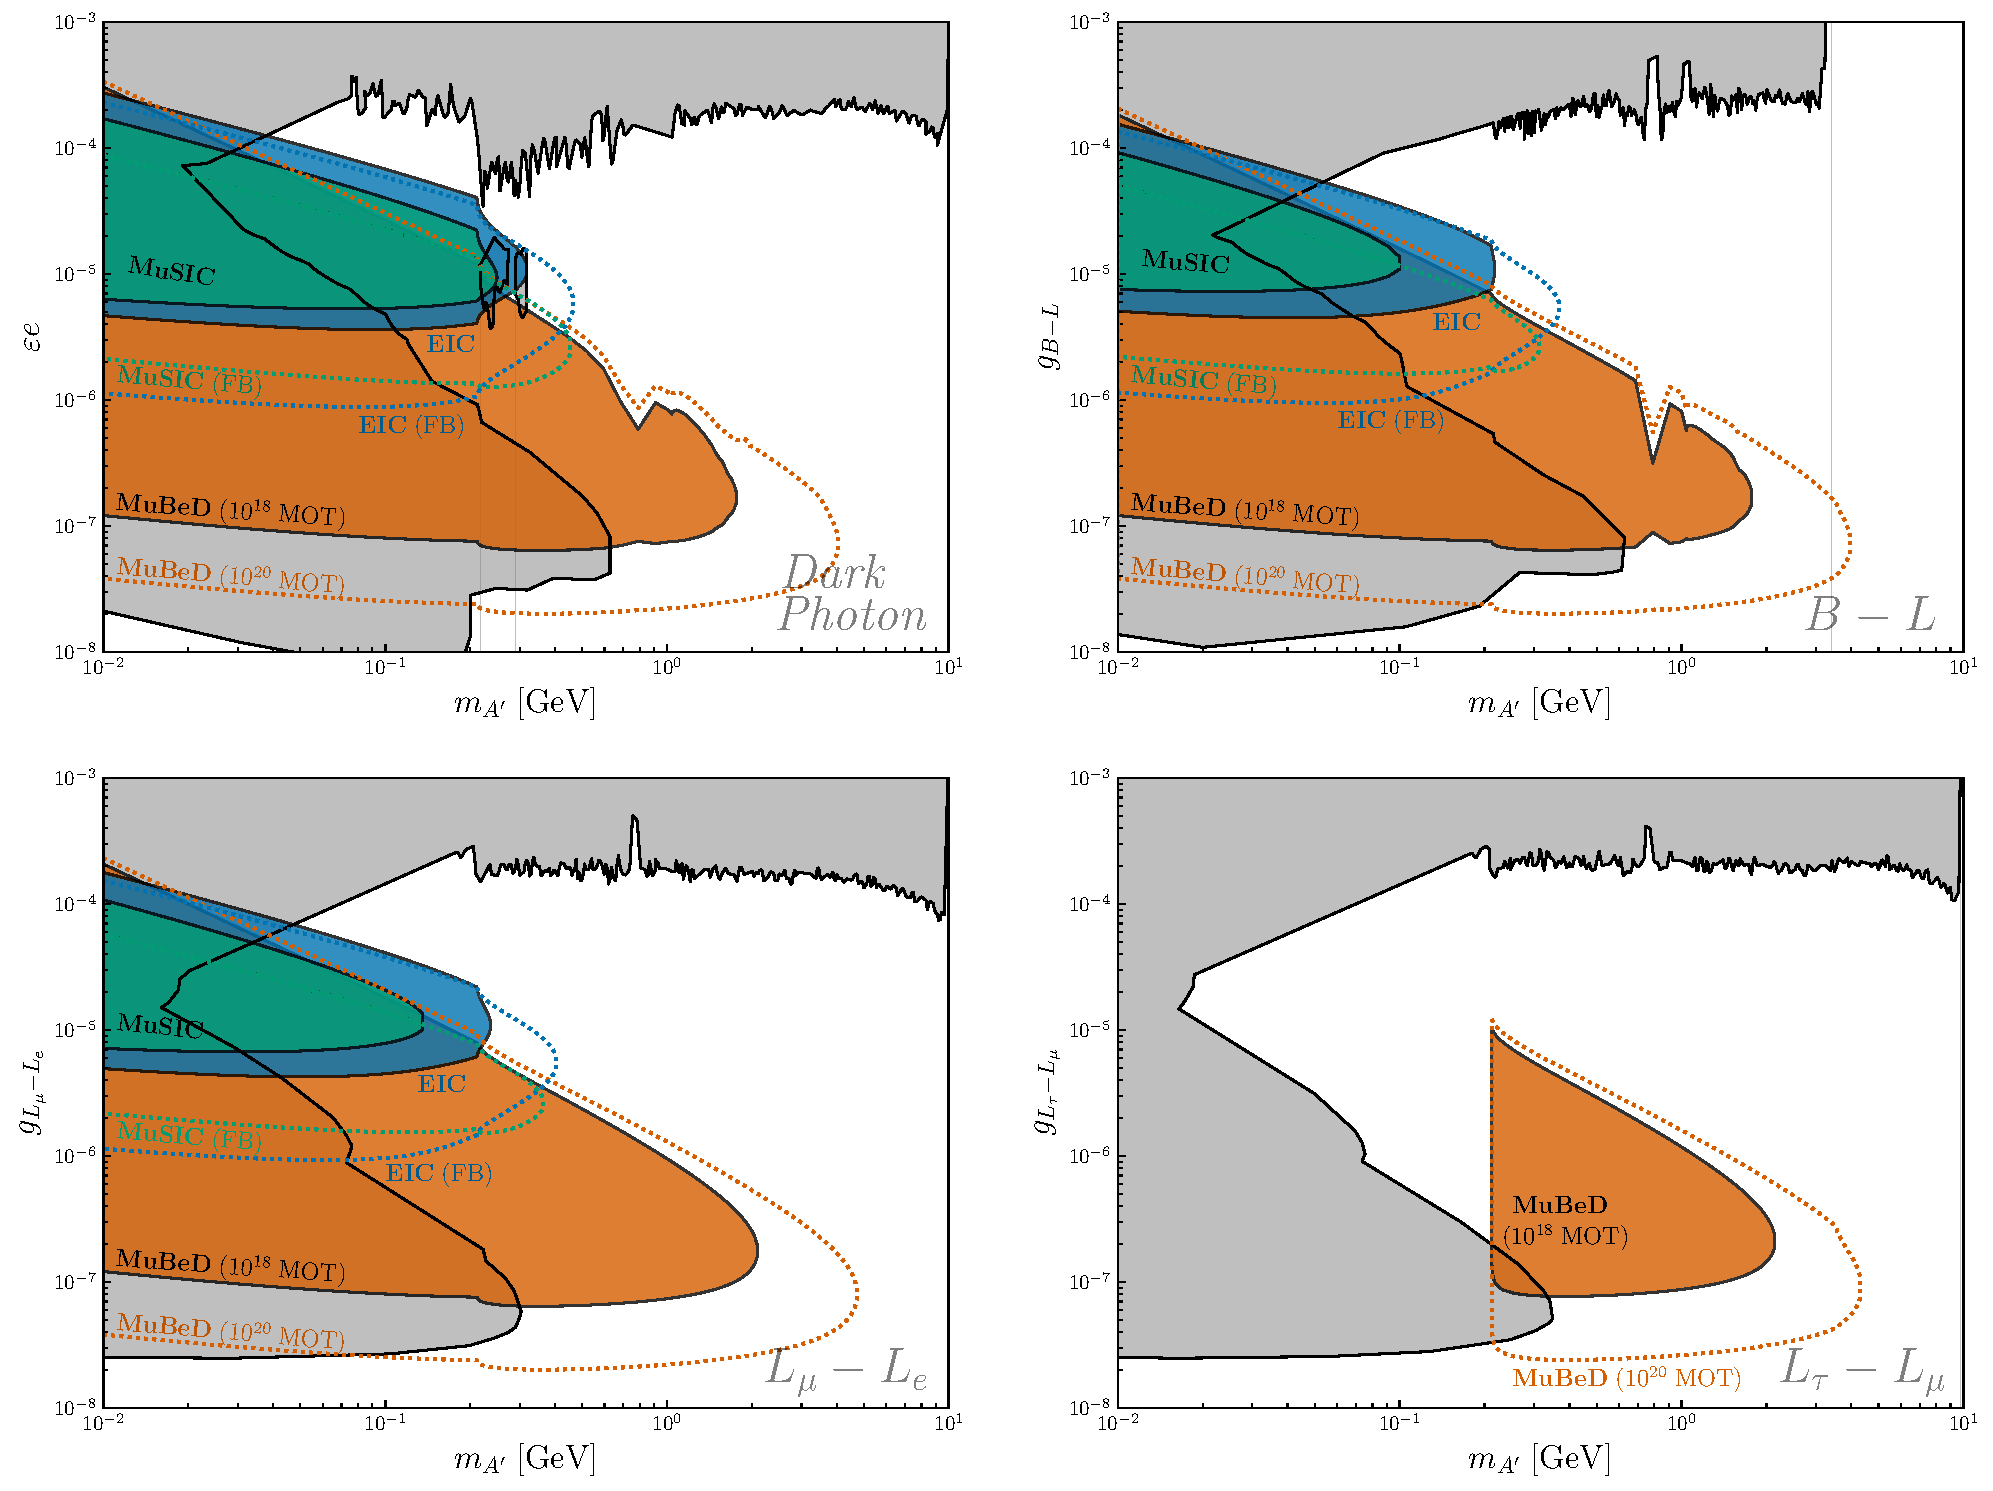
\includegraphics[width=\linewidth]{figures/chapter6/dark_bosons_MuBeD_MuSIC.pdf}
    \caption[Projected constraints at the EIC, MuBeD, and MuSIC on the kinetic mixing of a dark photon and gauge strength of anomaly-free abelian theories.]{Projected constraints at the EIC, MuBeD, and MuSIC on the kinetic mixing of a dark photon (top left) and gauge strength of the anomaly-free abelian theories $U(1)_{B-L}$ (top right), $U(1)_{L_\mu - L_e}$ (bottom left) and $U(1)_{L_\tau - L_\mu}$ (bottom right). To avoid clutter, we only show prior constraints, and no projections from other future experiments. An explanation of the exclusion limits is given in the caption of Fig.~\ref{fig:dark_bosons_EIC}. A comprehensive list of projections can be found in Ref.~\cite{Bauer:2018onh}. Our results for the dark photon and $L_\tau - L_\mu$ are in agreement with Ref.~\cite{Cesarotti:2022ttv}.}
    \label{fig:dark_bosons_MuBeD_MuSIC}
\end{figure}



\section{Limits at MuBeD and MuSIC}\label{sec:vector_MuBeD_MuSIC_limits}

To place $95\%$ C.L. limits at MuBeD and MuSIC, we once again compute those values of $g_X$ for which $N_{\rm sig.}(g_X) > 3.09$. The results are shown alongside the EIC projected constraints in Fig.~\ref{fig:dark_bosons_MuBeD_MuSIC}. The MuSIC results are shown in green, and the MuBeD results are shown in orange.  MuBeD and MuSIC are not sensitive to $L_\tau - L_e$, but are potentially sensitive to $L_\tau - L_\mu$. Hence, we show the results for $L_\tau-L_\mu$ instead (bottom right), alongside the results for the dark photon (top left), $B-L$ (top right), and $L_\mu - L_e$ (bottom left). As with the EIC, results for MuSIC are presented for two scenarios: a pseudo-rapidity coverage of $-6 < \eta < 6$, and a wider ``far-backward'' coverage of $|\eta| < 8$. 

Surprisingly, MuSIC does not appear to be competitive with the EIC, despite the additional energy of the muon beam. Part of the reason for this is the large pseudo-rapidity of the produced bosons at MuSIC. As a result, only the far-backward coverage of MuSIC is competitive with the EIC, because most particles produced have a pseudo-rapidity $|\eta| > 6$. In addition, it is important to note that while the available energy is higher at MuSIC than the EIC (with a muon beam energy of $E_{\rm MuSIC} \approx 20~{\rm TeV}$ in the ion frame at the MuSIC as opposed to an electron beam energy of $E_{\rm EIC} \approx 4~{\rm TeV}$ in the ion frame at the EIC), a look at Fig.~\ref{fig:production_crossx} reveals that the cross-section for on-diagonal production at MuSIC is smaller than that at the EIC for $m_{A'} \lesssim m_\mu$. This can be understood in the WW approximation from the fact that most of the cross-section is sampled near the minimum possible photon transfer $t_{-} \sim [m_\varphi (2m_\ell + m_\varphi)/2E]^2$, and scales as $\sigma \sim 1/t^2$. While $E$ is larger at MuSIC than the EIC, the numerator for $m_\varphi < m_\mu$ is $[m_\varphi (2m_\mu + m_\varphi)]^2 \sim 4m_\varphi^2 m_\mu^2$ at MuSIC, but $[m_\varphi(2m_e + m_\varphi)]^2 \sim m_\varphi^4$ at the EIC. Hence, $t_-$ is ultimately suppressed at the EIC relative to MuSIC, making the resulting production cross-section larger. While MuSIC is technically sensitive to $U(1)_{L_\tau - L_\mu}$ gauge bosons, we find that given our assumptions, the sensitivity is too weak to provide meaningful limits.

 MuBeD, on the other hand, is competitive over the entire range of couplings, for both $N_\mu = 10^{18}$ and $N_\mu = 10^{20}$ muons on target. This result highlights the advantage of beam dump experiments over lepton-ion colliders: a higher luminosity (by virtue of the dense target) and increased pseudorapidity coverage (capturing all particles with $\eta \gtrsim 5$). While lepton-ion colliders can peripherally produce higher-mass particles than their beam-dump counterparts (which is what allows the EIC to compete with past beam-dump experiments), this effect is not enough to give MuSIC or the EIC an edge over a $1~{\rm TeV}$ muon beam dump. The rate of production for GeV-scale particles, and their corresponding lab-frame lifetimes, are just too low for either experiment to provide meaningful displaced limits at this mass range. 

\section{Displaced Vertex Resolution Considerations}\label{sec:displaced_vertex_resolution}

The analysis for the EIC and MuSIC above notably relied on the assumption that the reconstructed tracks of the vector boson final states were straight-line trajectories. Here we will evaluate the sensitivity of this analysis to the details of the reconstructed trajectory. In particular, we will consider two alternative analyses: one will estimate the effect of an external magnetic field of $1~{\rm T}$, and the other will completely discard the transverse DCA analysis in favor of a simpler fiducial $d_{\rm min}$, which is independent of the kinematics of the final-state particle.


\begin{figure}[t!]
    \centering
    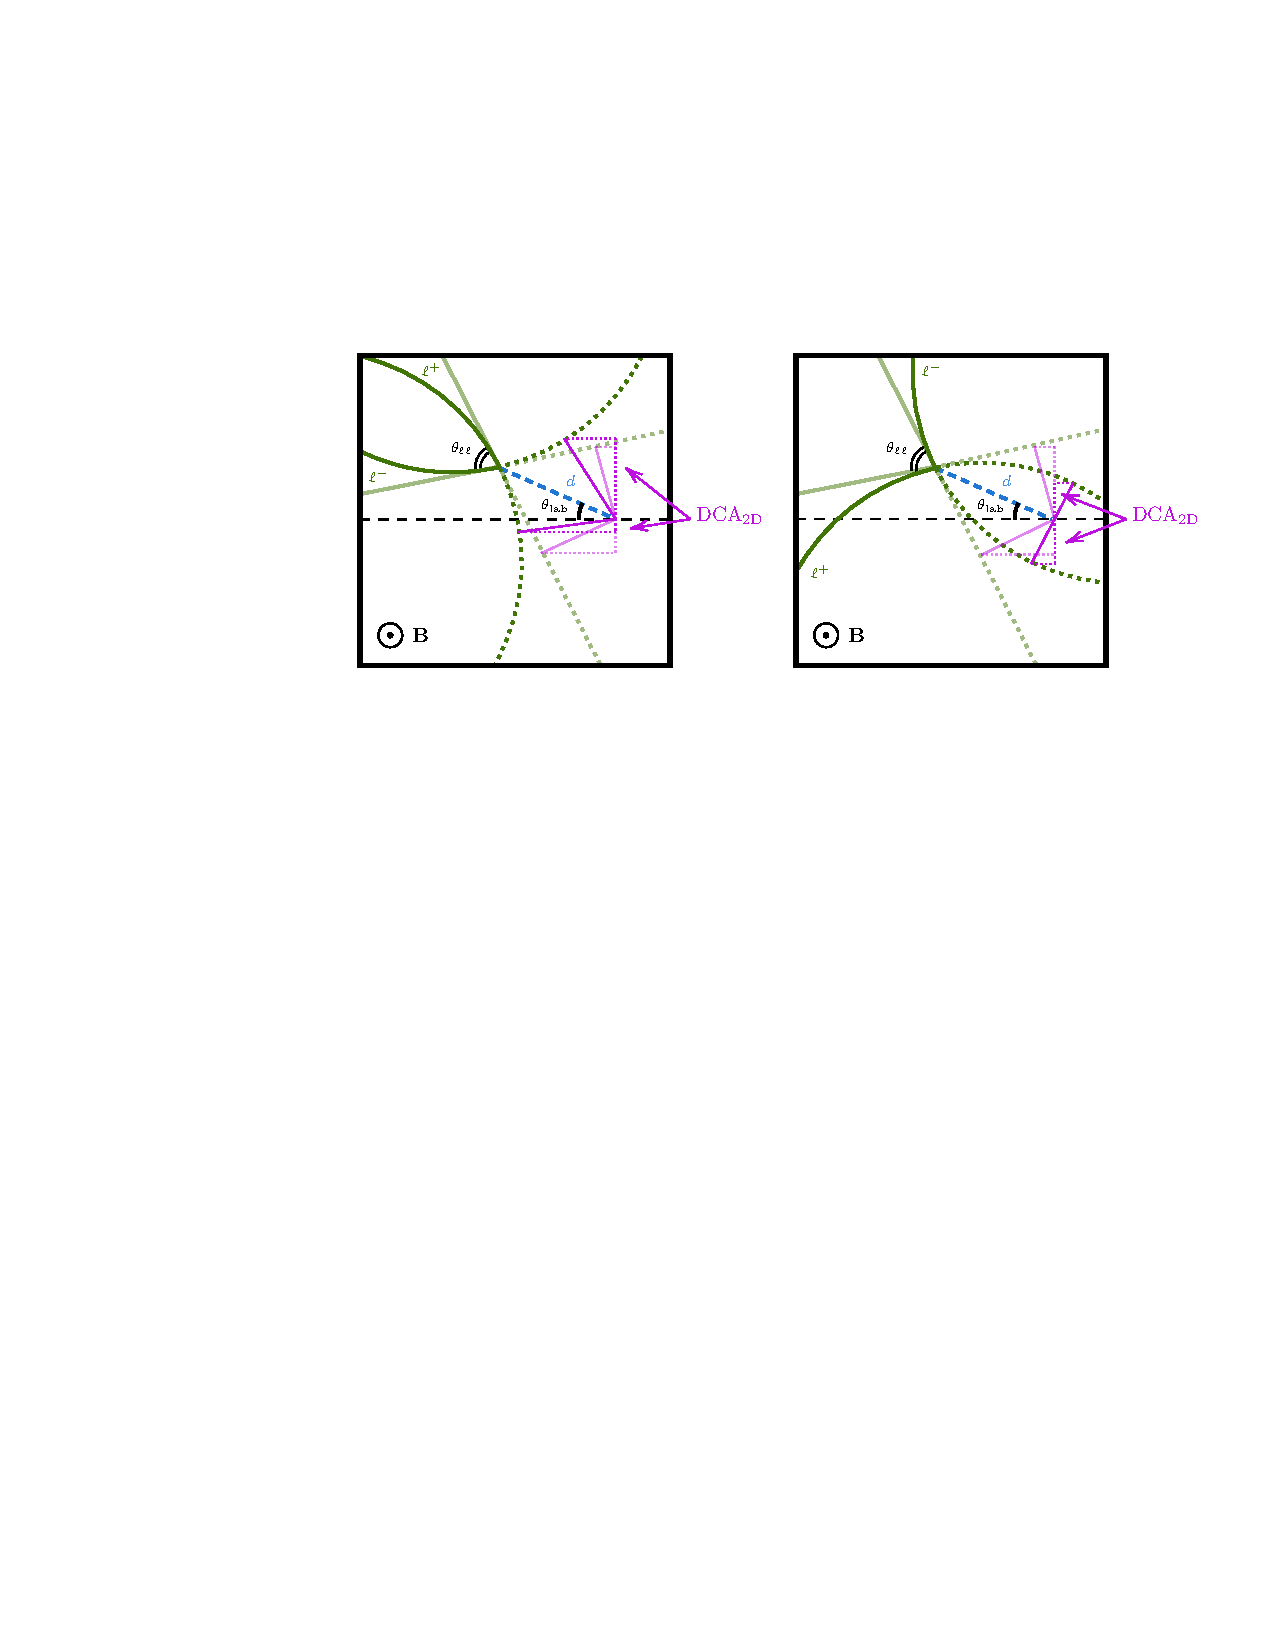
\includegraphics[width=\linewidth]{figures/chapter6/Bfield.pdf}
    \caption[A schematic representation of the difference between the transverse DCAs for a straight-line reconstructed trajectory and a circular reconstructed trajectory.]{A schematic representation of the difference between the transverse DCAs for a straight-line reconstructed trajectory and a circular reconstructed trajectory (consistent with the final-state leptons being immersed in a uniform magnetic field {\bf B}). The diagrams on the left and right demonstrate the two possible in-plane orientations of the $\ell^+$ relative to the $\ell^-$.}
    \label{fig:BfieldDCA}
\end{figure}


To estimate the sensitivity of the analysis to deviations in a straight-line trajectory, we consider the scenario where the final-state leptons experience a uniform magnetic field ${\bf B}$ with magnitude $1~{\rm T}$ (which is the anticipated strength of the magnets at the EIC \cite{Adkins:2022jfp}). For simplicity, we assume that the leptonic decay products of the $A'$ are always in the plane perpendicular to the magnetic field, so that their reconstructed tracks are circular arcs of radius $R_B = E_\ell v/eBc$. This assumption is far from realistic, but represents the {\it maximal} deviation from a straight-line trajectory one can expect either of the leptonic final states to follow. Hence, this analysis will be a useful metric for evaluating the validity of our initial assumption of a straight-line trajectory. A schematic representation of this set-up is shown in Fig.~\ref{fig:BfieldDCA}. For simplicity, we assume that each final-state lepton has an initial direction at an angle of $\theta_{\ell\ell}/2 \approx m_{A'}/E_{A'}$ w.r.t. the direction of the boson. We consider both possible orientations of in-plane final states (i.e., whether the $\ell^+$ is clockwise or counterclockwise from the $\ell^-$) and assume that each of these occurs for 50\% of produced events. For each orientation, we compute the average transverse DCA of both final-states  $\overline{{\rm DCA}_{\rm 2D}}$, and only count those events for which $\overline{{\rm DCA}_{\rm 2D}} > {\rm DCA}_{\rm 2D}^{\rm min}$. 


We would also like to assess how much the analysis differs if we choose a fiducial minimum displacement $d_{\rm min}$ in Eq.~\ref{eq:pdisp}. For both the EIC and MuSIC, we assume that $d_{\rm min} = 1~{\rm cm}$. This is a relatively large displacement, so it may seem like a reasonable assumption given the sensitivity of modern detectors. However, when the opening angle of the final-state lepton pair is small, it can be difficult to discern exactly where the leptons originated, which is why the transverse DCA is likely a more reliable metric for resolving displacements.


\begin{figure}[t!]
    \centering
    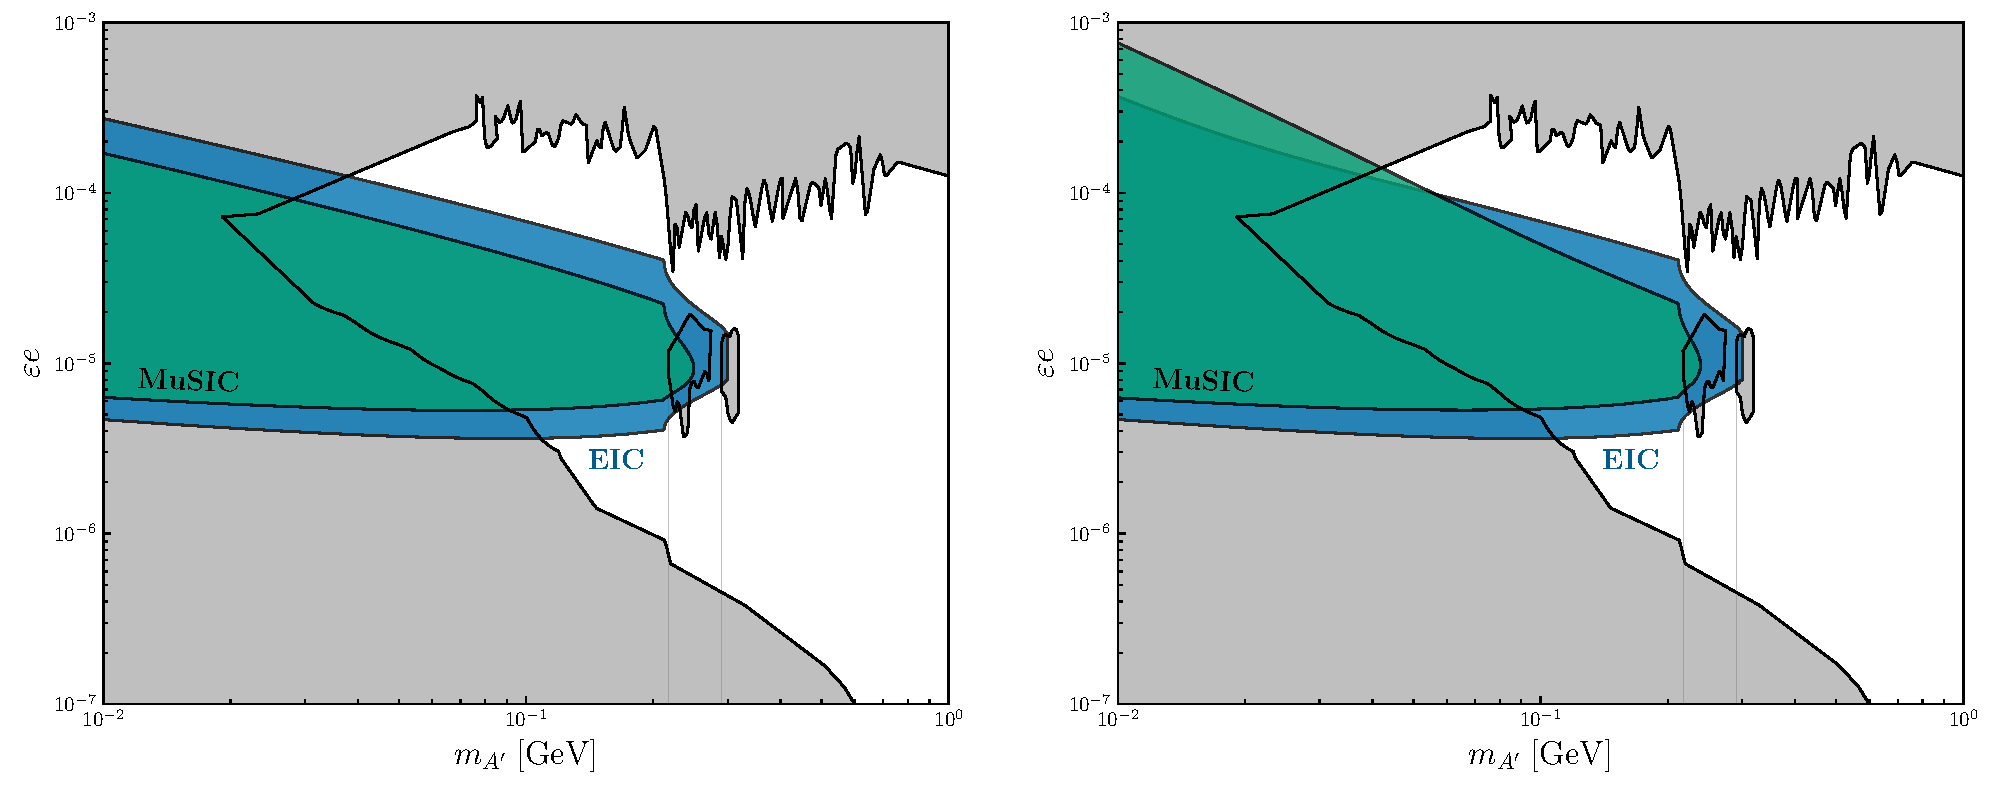
\includegraphics[width=\linewidth]{figures/chapter6/dark_bosons_B_field_analysis.pdf}
    \caption[Limits on the dark photon kinetic mixing $\varepsilon e$ under different analyses.]{Limits on the dark photon kinetic mixing $\varepsilon e$ assuming each final-state lepton is deflected by a $1~{\rm T}$ magnetic field (left) and assuming a fiducial minimum displacement of $d_{\rm min} = 1~{\rm cm}$ (right). Limits from the EIC are shown in blue, and limits from MuSIC are shown in green.}
    \label{fig:alt_analysis}
\end{figure}

Projected exclusions on the kinetic mixing of a dark photon at the EIC and MuSIC for both of these analyses are shown in Fig.~\ref{fig:alt_analysis}. The limits from the $B$-field analysis shown in the left panel and limits from the fiducial $d_{\rm min}$ analysis shown in the right panel. The addition of a large transverse magnetic field has minimal effect on the results found in Section \ref{sec:vector_MuBeD_MuSIC_limits}. The only difference appears for low masses ($m_{A'} = {\cal O}(10~{\rm MeV})$) and large couplings ($g_{A'} \sim 10^{-4}$--$10^{-3}$), in a region that is already mostly excluded by existing experiments. This aligns with the understanding that lower-mass particles do not carry away as much energy from the interaction, which results in a reduced energy for the final-state decay products. This in turn causes small turning radius in the magnetic field, which leads to a more drastic deviation from the straight-line trajectory scenario. The effect all but vanishes for larger masses at both experiments.  By contrast, we see that use of a fiducial minimum displacement $d_{\rm min} = 1~{\rm cm}$ has a profound effect on the projected exclusions, especially for MuSIC. Hence, if other experimental methods can be used to identify displacements, they would have the potential to drastically improve the reach of these experiments. In addition, we note that limits at both the EIC and MuSIC can be improved with a better DCA resolution.


